%
% Chapter on Curve fitting
%
% (c) 2012 Prof Dr Andreas Mueller, Hochschule Rapperswil
% $Id$
\subsection{Kurvenanpassung}
\begin{figure}
\begin{center}
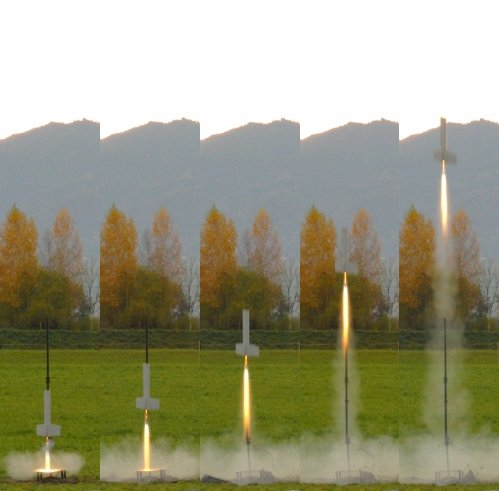
\includegraphics[width=0.6\hsize]{graphics/stummel}
\end{center}
\caption{Bildsequenz Raketenstart, Interval zwischen den Bildern: $\frac1{30}$s.
\label{stummel}}
\end{figure}
In der Praxis hat man h"aufig mit Messdaten zu tun, die mit einem
bekannten Naturgesetz in Einklang gebracht werden sollen.
Abbildung~\ref{stummel} zeigt den Start einer Rakete, es ist
bekannt, dass sich diese bei konstanter Beschleunigung nach dem
Gesetz
\[
s(t)=s_0+v_0t+\frac12a_0t^2
\]
bewegen wird. Wie gross ist die Beschleunigung $a_0$?
Die Schwierigkeit besteht darin, dass es offenbar nicht zul"assig ist
anzunehmen, die Rakete sei beim ersten Bild in Ruhe ($v_0=0$ oder
$s_0=0$). Es m"ussen also alle drei Unbekannten $a_0$, $v_0$
und $s_0$ miteinander bestimmt werden.

\subsubsection{Lineare Regression}
Zur Einf"uhrung behandeln wir den Fall einer Geraden. Wir gehen also
davon aus, dass zwischen den Gr"ossen $x$ aund $y$ ein linearer
Zusammenhang
\[
y=a_1x+a_0
\]
besteht. Ausserdem sind $n$ Messungen von $x$ und $y$ gemacht worden,
wir nennen die Messwerte $x_i$ und $y_i$, $1\le i\le n$. Wir haben 
jetzt also $n$ lineare Gleichungen
\[
\begin{linsys}{3}
a_0&+&x_1a_1&=&y_1\\
\vdots& &   & &\vdots\\
a_0&+&x_na_1&=&y_n\\
\end{linsys}
\]
f"ur die beiden Unbekannten $a_0$ und $a_1$.
Mit der Schreibweise von Abschnitt~\ref{section:ueberbestimmt} haben wir eine
"uberbestimmtes Gleichungssystem mit
\[
A=\begin{pmatrix}
x_1&1\\
x_2&1\\
\vdots&\vdots\\
x_n&1
\end{pmatrix},\qquad
b=\begin{pmatrix}
y_1\\y_2\\\vdots\\y_n
\end{pmatrix},\qquad
x=\begin{pmatrix}
a_1\\a_0
\end{pmatrix}.
\]
Nach (\ref{uberbestimmt}) ist der gesuchte Vektor $a$ die L"osung
eines Gleichungssystems mit Koeffizientenmatrix
\[
A^tA=\begin{pmatrix}
\sum_{i=1}^nx_i^2&\sum_{i=1}^nx_i\\
\sum_{i=1}^nx_i&n
\end{pmatrix}
\]
und rechter Seite
\[
A^tb=\begin{pmatrix}
\sum_{i=1}^nx_iy_i\\
\sum_{i=1}^ny_i
\end{pmatrix}.
\]
Mit der Cramerschen Regel kann man dieses sofort l"osen. Der gemeinsame
Nenner ist 
\[
\det(A^tA)=n\sum_{i=1}^nx_i^2-\biggl(\sum_{i=1}^nx_i\biggr)^2,
\]
und die L"osungen sind
\begin{align}
a_1
&=
\frac{n\sum_{i=1}^nx_iy_i-\sum_{i=1}^n x_i\sum_{i=1}^ny_i}%
{n\sum_{i=1}^nx_i^2-\bigl(\sum_{i=1}^nx_i\bigr)^2}
=
\frac{\frac1n\sum_{i=1}^nx_iy_i-\bigl(\frac1n\sum_{i=1}^n x_i\bigr)\bigl(\frac1n \sum_{i=1}^ny_i\bigr)}%
{\frac1n\sum_{i=1}^nx_i^2-\bigl(\frac1n\sum_{i=1}^nx_i\bigr)^2}
\label{regression:steigung}
\\
a_0
&=
\frac{\sum_{i=1}^nx_i^2\sum_{i=1}^n y_i-\sum_{i=1}^n x_iy_i\sum_{i=1}^n x_i }%
{n\sum_{i=1}^nx_i^2-\bigl(\sum_{i=1}^nx_i\bigr)^2}
\notag
\\
&=
\frac{\bigl(\frac1n\sum_{i=1}^nx_i^2\bigr)\bigl(\frac1n\sum_{i=1}^n y_i\bigr)
-\bigl(\frac1n\sum_{i=1}^n x_iy_i\bigr)\bigl(\frac1n\sum_{i=1}^n x_i\bigr) }%
{\frac1n\sum_{i=1}^nx_i^2-\bigl(\frac1n\sum_{i=1}^nx_i\bigr)^2}
\notag
\\
&=
\frac1n\sum_{i=1}^n y_i
-
a_1\biggl(\frac1n\sum_{i=1}^n x_i\biggr).
\label{regression:achsabschnitt}
\end{align}
Dabei haben wir die Br"uche durch $n^2$ gek"urzt, damit die Summen
etwas besser verst"andlich sind, 
$\frac1n\sum_{i=1}^nx_i$ ist der Mittelwert der $x$-Werte,
$\frac1n\sum_{i=1}^ny_i$ ist der Mittelwert der $y$-Werte.
Die Formeln (\ref{regression:steigung}) und (\ref{regression:achsabschnitt})
beschreiben eine Gerade mit Steigung $a_1$ und Achsabschnitt $a_0$,
die optimal an die Messdaten angepasst ist.

\subsubsection{Anpassung an ein Polynom}
Nach dem gleichen Schema kann jetzt ein beliebiges Polynom
\[
a_0+a_1x+a_2x^2+\dots+a_mx^m
\]
an die Daten angepasst werden. Gesucht ist der Vektor der Koeffizienten
$a_k$, welcher am besten an die Messdaten $(x_i,x_i)$, $1\le i\le n$
angepasst ist. Wie im vorangegangen Abschnitt m"ussen wir also eine
optimale L"osung f"ur das "Uberbestimmte Gleichungsystem
\[
\begin{linsys}{6}
a_0&+&a_1x_1&+&a_2x_1^2&+&\dots &+&a_mx_1^m&=&y_1\\
a_0&+&a_1x_2&+&a_2x_2^2&+&\dots &+&a_mx_2^m&=&y_2\\
\vdots   & &      & &        & &\ddots& &\vdots  & &\vdots\\
a_0&+&a_1x_n&+&a_2x_n^2&+&\dots&+&a_mx_n^m&=&y_n\\
\end{linsys}
\]
Mit der Koeffizientenmatrix und rechter Seite
\[
A=\begin{pmatrix}
1&x_1&x_1^2&\dots&x_1^m\\
1&x_2&x_2^2&\dots&x_2^m\\
\vdots&\vdots&\vdots&\ddots&\vdots\\
1&x_n&x_n^2&\dots&x_n^m
\end{pmatrix},\qquad
b=\begin{pmatrix}y_1\\y_2\\\vdots\\y_m\end{pmatrix}.
\]
Wiederum gilt
\[
a=(A^tA)^{-1} A^tb,
\]
Die Matrix $A^tA$ und der Vektor $A^tb$ sind leicht zu berechnen
\begin{align*}
A^tA&=\begin{pmatrix}
n                &\sum_{i=1}^nx_i      &\sum_{i=1}^nx_i^2    &\dots &\sum_{i=1}^nx_i^m\\
\sum_{i=1}^nx_i  &\sum_{i=1}^nx_i^2    &\sum_{i=1}^nx_i^3    &\dots &\sum_{i=1}^nx_i^{m+1}\\
\sum_{i=1}^nx_i^2&\sum_{i=1}^nx_i^3    &\sum_{i=1}^nx_i^4    &\dots &\sum_{i=1}^nx_i^{m+2}\\
\vdots           &\vdots               &\vdots               &\ddots&\vdots\\
\sum_{i=1}^nx_i^m&\sum_{i=1}^nx_i^{m+1}&\sum_{i=1}^nx_i^{m+2}&\dots &\sum_{i=1}^nx_i^{2m}
\end{pmatrix}
,\qquad
A^tb=\begin{pmatrix}
\sum_{i=1}^ny_i     \\
\sum_{i=1}^ny_ix_i  \\
\sum_{i=1}^ny_ix_i^2\\
\vdots\\
\sum_{i=1}^ny_ix_i^m
\end{pmatrix}
\end{align*}
Meist wird man aber beide Seiten durch $n$ teilen, dadurch k"onnen die
Matrixelemente wieder als Mittelwerte interpretiert werden:
\begin{equation}
\begin{pmatrix}
a_0\\
a_1\\
a_2\\
\vdots\\
a_m
\end{pmatrix}
=
\begin{pmatrix}
1
	&\frac1n\sum_{i=1}^nx_i
		&\frac1n\sum_{i=1}^nx_i^2
			&\dots
				&\frac1n\sum_{i=1}^nx_i^m\\
\frac1n\sum_{i=1}^nx_i
	&\frac1n\sum_{i=1}^nx_i^2
		&\frac1n\sum_{i=1}^nx_i^3
			&\dots
				&\frac1n\sum_{i=1}^nx_i^{m+1}\\
\frac1n\sum_{i=1}^nx_i^2
	&\frac1n\sum_{i=1}^nx_i^3
		&\frac1n\sum_{i=1}^nx_i^4
			&\dots
				&\frac1n\sum_{i=1}^nx_i^{m+2}\\
\vdots
	&\vdots
		&\vdots
			&\ddots
				&\vdots\\
\frac1n\sum_{i=1}^nx_i^m
	&\frac1n\sum_{i=1}^nx_i^{m+1}
		&\frac1n\sum_{i=1}^nx_i^{m+2}
			&\dots
				&\frac1n\sum_{i=1}^nx_i^{2m}
\end{pmatrix}^{-1}
\begin{pmatrix}
\frac1n\sum_{i=1}^ny_i     \\
\frac1n\sum_{i=1}^ny_ix_i  \\
\frac1n\sum_{i=1}^ny_ix_i^2\\
\vdots\\
\frac1n\sum_{i=1}^ny_ix_i^m
\end{pmatrix}
\label{polynomregression}
\end{equation}
Die Matrixelemente sind wieder Mittelwerte der Potenzen der Messwerte.

\subsubsection{Beschleunigung der Rakete}
Wir wenden die Formel~(\ref{polynomregression}) auf die startende 
Rakete an. Die Werte $x_i$ und $y_i$ kann man aus dem Bild herauslesen.
Die Zeitabst"ande zwischen den Fotos sind $0.033333$s, die L"ange der
Rakete ist 75cm oder 48 Pixel, durch Ausz"ahlen der Pixel kann man
die H"ohe der Rakete in Meter umrechnen:
\begin{center}
\begin{tabular}{|>{$}r<{$}|>{$}c<{$}>{$}c<{$}|}
\hline
i&x_i&y_i\\
\hline
1&0.033333& 0.00000\\
2&0.066667& 0.42188\\
3&0.100000& 1.28125\\
4&0.133333& 2.57812\\
5&0.166667& 4.32812\\
\hline
\end{tabular}
\end{center}
Aus diesen Daten kann man jetzt die Matrix $A$ und den Vektor $b$
konstruieren:
\[
A=\begin{pmatrix}
   1 & 0.0333333 & 0.0011111\\
   1 & 0.0666667 & 0.0044444\\
   1 & 0.1000000 & 0.0100000\\
   1 & 0.1333333 & 0.0177778\\
   1 & 0.1666667 & 0.0277778
\end{pmatrix}
,\qquad
b=\begin{pmatrix}
   0.00000\\
   0.56250\\
   1.70833\\
   3.43750\\
   5.77083
\end{pmatrix}
\]
Zur Bestimmung von $a$ muss man jetzt $A^tA$ und $A^tb$ berechnen:
\[
A^tA=\begin{pmatrix}
   5.0000000&  0.5000000&  0.0611111\\
   0.5000000&  0.0611111&  0.0083333\\
   0.0611111&  0.0083333&  0.0012086
\end{pmatrix},\qquad
A^tb=\begin{pmatrix}
   8.60938\\
   1.22135\\
   0.18075
\end{pmatrix}
\]
Die L"osung des Gleichungssystems ist damit
\[
a=(A^tA)^{-1}A^tb=
\left(
\begin{matrix}
\begin{tabular}{r}
   0.0250\\
  -7.3393\\
   198.88
\end{tabular}
\end{matrix}
\right)
\]
Die dazugeh"orige Kurve passt sehr gut ins Bild: \ref{stummel2}.
Hier kann man ablesen, dass $a_2=198.88\frac{\text{m}}{\text{s}}$, was
etwa $40.5g$ entspricht.

Wegen $v=a_1+2a_2t$ kann man jetzt auch die Startzeit ausrechnen,
sie erf"ullt $a_1+2a_2t=0$, also $t=-a_1/2a_2=0.018451$,  der
Start erfolgte also $0.014882$s vor dem ersten Foto.
\begin{figure}
\begin{center}
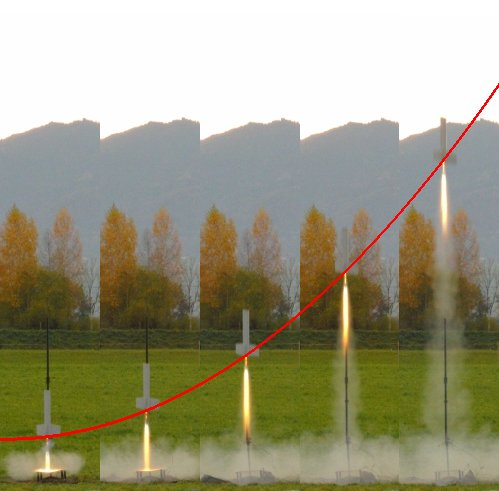
\includegraphics[width=0.6\hsize]{graphics/stummel2}
\end{center}
\caption{Bildsequenz Raketenstart mit angepasster Parabel $s=a_0+a_1t+a_1t^2$.
\label{stummel2}}
\end{figure}

\subsubsection{Weitere Funktionen}
Auch f"ur andere Funktionen kann das Verfahren eine Anpassung bringen.
Allerdings muss sichergestellt sein, dass die zu bestimmenden Koeffizienten
linear eingehen. So kann man zum Beispiel die Funktion
\[
f(x)=a_0e^{a_1x}
\]
nicht direkt anpassen, weil der Koeffizient $a_1$ nicht linear eingeht.
Wenn man aber von den $y$-Werten den Logarthimus nimmt, bekommt man
\[
\log f(x)=\log a_0+a_1 x
\]
Linear Regression f"ur die Daten $(x_i,\log y_i)$ liefert die Koeffizienten
$\log a_0$ und $a_1$. Die folgende Tabelle zeigt, welche Funktionen durch
diese einfach Modifikation behandelt werden k"onnen. Die Spalte 
``Daten'' enth"alt zeigt, auf welche Daten der Algorithmus angewendet
werden muss, um die Koeffizieten in der Spalte ``Koeffizienten''
zu liefern.
\begin{center}
\begin{tabular}{>{$}c<{$}>{$}c<{$}>{$}c<{$}>{$}c<{$}}
\hline
f(x)              &\log f(x)         & \text{Daten}      &\text{Koeffizienten}\\
\hline
a_0+a_1x          &                  &(x_i,y_i)          &a_0, a_1\\
a_0e^{a_1x}       &\log a_0+a_1 x    &(x_i,\log y_i)     &\log a_0, a_1 \\
a_0x^{a_1}        &\log a_0+a_1\log x&(\log x_1,\log y_i)&\log a_0, a_1 \\
a_0 + a_1\log x   &                  &(\log x_1,y_i)     &a_0, a_1 \\
\hline
\end{tabular}
\end{center}
